\documentclass[handout, aspectratio=169, notes=hide]{beamer}

\usepackage{attrib}
\graphicspath{{./figures/}}
\DeclareGraphicsExtensions{.pdf,.jpeg,.png,.jpg}
\usepackage[export]{adjustbox}
\usepackage{eurosym}
\usepackage{xcolor}
\usepackage{textpos}
\usepackage{turnstile}
\usepackage{listings}

\def\UrlBreaks{\do\/\do-}
\newcommand{\nc}{\,\mid\!\sim\,}

\usetheme{Rochester}
\usecolortheme{beaver}

\definecolor{pico}{RGB}{240,145,70}
\definecolor{darkorange}{RGB}{212,101,11}

%\setbeamercolor{frametitle}{fg=darkorange}
%\setbeamercolor{title}{fg=darkorange}
%\setbeamercolor{structure}{fg=pico}

\setbeamertemplate{bibliography entry title}{}
\setbeamertemplate{bibliography entry location}{}
\setbeamertemplate{bibliography entry note}{}

\renewcommand{\thefootnote}{\fnsymbol{footnote}}
\newcommand{\prescite}[1]{\footnote{\cite{#1}}}
\newcommand{\prestext}[1]{\footnotetext{\cite{#1}}}
\usepackage{perpage}
\MakePerPage{footnote}

\def\etal{{\it et al.}}
\def\etc{{\it etc.}}
\def\eg{{\it e.g.}}
\def\ie{{\it i.e.}}
\def\cf{{\it cf.}}
\def\qv{{\it q.v.}}
\def\qqv{{\it qq.v.}}
\def\st{s.t.\ }
\def\concat{\mathbin{|}}
\def\vs{{\it vs.}}

\begin{document}

\titlegraphic{
\begin{textblock*}{250mm}(-0.5cm,-7.5cm)
\smash{
\includegraphics[width=0.13\textwidth]{camlogo}}
\end{textblock*}
\begin{textblock*}{250mm}(13.2cm,-7.3cm)
\smash{
\includegraphics[width=0.05\textwidth]{raven-logo}}
\end{textblock*}
}

\addtobeamertemplate{frametitle}{}{%
\begin{textblock*}{250mm}(0.8\textwidth,-1.25cm)

\includegraphics[width=0.13\textwidth]{camlogo}
\end{textblock*}
}


\title{Raven Authentication Service}
\subtitle{Attacks and Countermeasures}
\author{Graham Rymer \and David Llewellyn-Jones}
\institute{University of Cambridge, Computer Laboratory,\\
William Gates Building, 15 JJ Thomson Avenue,\\
Cambridge CB3 0FD, UK \\
\quad \\
\href{mailto:Graham.Rymer@cl.cam.ac.uk}{Graham.Rymer@cl.cam.ac.uk}\\
\href{mailto:David.Llewellyn-Jones@cl.cam.ac.uk}{David.Llewellyn-Jones@cl.cam.ac.uk}\\
}
\date{19th March 2018}

%%%%%%%%%%%%%%%%%%%%%%%%%%%%%%%%%%%%%%%%%

\frame{\titlepage}
\note{

}

%%%%%%%%%%%%%%%%%%%%%%%%%%%%%%%%%%%%%%%%%

\begin{frame}
\frametitle{Raven}
\framesubtitle{What is Raven}
\setlength{\parskip}{1.0em}
\centering
\begin{columns}[T]
\begin{column}[T]{0.5\textwidth}
\begin{enumerate}
\setlength{\parskip}{1.0em}
\item Single-Sign On
\item Authentication by username and password
\item Initially approved 2002
\item Identity provider for all students and staff
\item Only used within University of Cambridge
\end{enumerate}
\end{column}
\begin{column}[T]{0.5\textwidth}
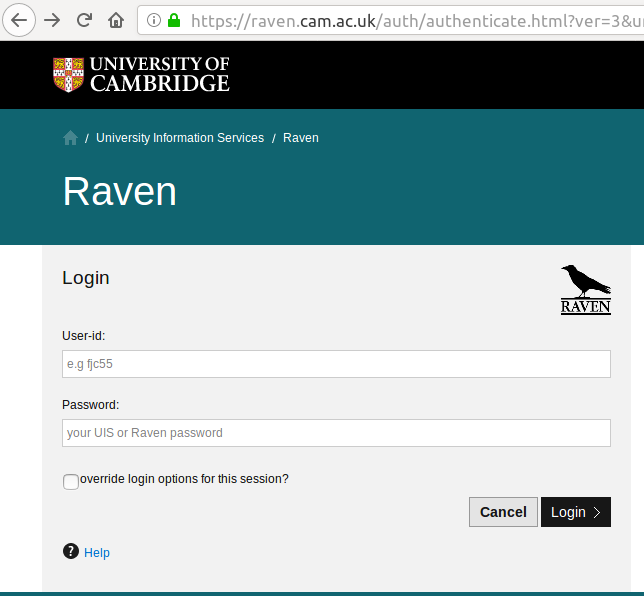
\includegraphics[width=1.0\textwidth,right]{raven-login}
\end{column}
\end{columns}

\end{frame}
\note{
}

%%%%%%%%%%%%%%%%%%%%%%%%%%%%%%%%%%%%%%%%%

\begin{frame}
\frametitle{Raven}
\framesubtitle{What is Raven}
\setlength{\parskip}{1.0em}
\centering
\begin{columns}[T]
\begin{column}[T]{1.0\textwidth}
\setlength{\parskip}{1.0em}
Supports two protocols
\begin{enumerate}
\setlength{\parskip}{1.0em}
\item Ucam Webauth
\item Shibboleth (since 2007)
\end{enumerate}
We're primarily interested in Ucam Webauth
\end{column}
\end{columns}

\end{frame}
\note{
}

%%%%%%%%%%%%%%%%%%%%%%%%%%%%%%%%%%%%%%%%%

\begin{frame}
\frametitle{Raven Actors}
\framesubtitle{Actors involved in the authentication process}
\setlength{\parskip}{1.0em}
\centering
\begin{columns}[T]
\begin{column}[T]{1.0\textwidth}
\begin{enumerate}
\setlength{\parskip}{1.0em}
\item End user - The person being authenticated
\item WAA - Web Application Agent
\item WLS - Web Login Service
\item WB - Web Browser
\item Credential store - containing usernames and password hashes
\end{enumerate}
\end{column}
\end{columns}

\end{frame}
\note{
}

%%%%%%%%%%%%%%%%%%%%%%%%%%%%%%%%%%%%%%%%%

\begin{frame}
\frametitle{}
\framesubtitle{}
\setlength{\parskip}{1.0em}
\begin{columns}[T]
\begin{column}[T]{1.0\textwidth}	
\vspace{-1.7cm}
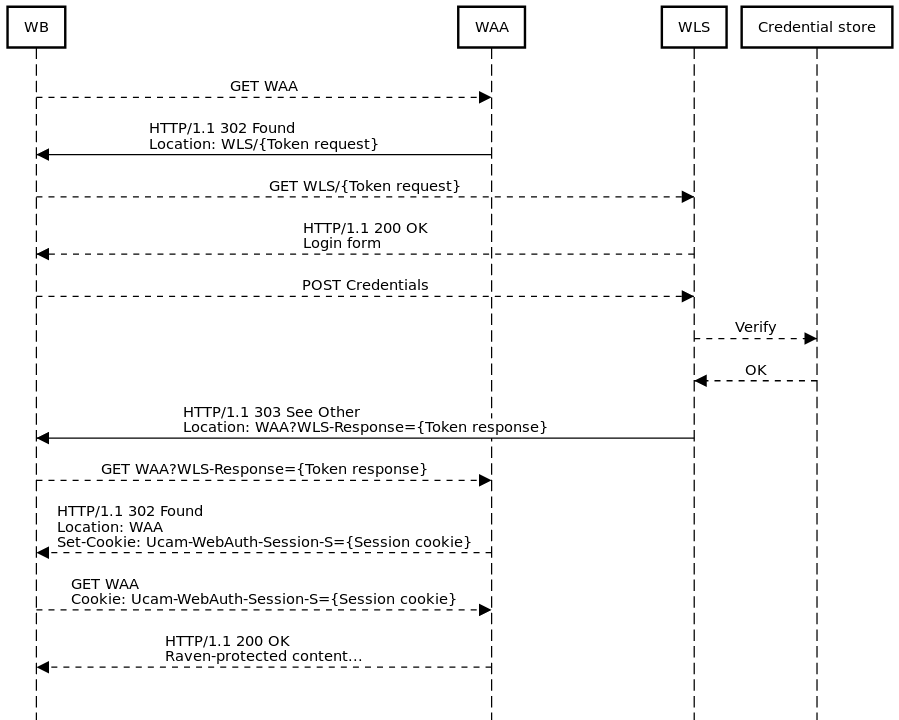
\includegraphics[width=0.76\textwidth,center]{ucam_webauth}
\end{column}
\begin{column}[T]{0.0\textwidth}
\end{column}
\end{columns}

\end{frame}
\note{
}

%%%%%%%%%%%%%%%%%%%%%%%%%%%%%%%%%%%%%%%%%

\begin{frame}
\frametitle{Message Space}
\framesubtitle{Protocol messages}
\setlength{\parskip}{1.0em}
\begin{columns}[T]
\begin{column}[T]{1.0\textwidth}	

\begin{align*}
\text{Token request} & := \mathit{ver} | \mathit{url} | \mathit{desc} | \mathit{aauth} | \mathit{iact} | \mathit{msg} | \mathit{params} | \mathit{date} | \mathit{skew} | \mathit{fail} \\
\text{Token response} & := \mathit{ver} | \mathit{status} | \mathit{msg} | \mathit{issue} | \mathit{id} | \mathit{url} | \mathit{principal} | \mathit{ptags} | \mathit{auth} | \mathit{sso} | \mathit{life} | {} \\
& \qquad \mathit{params} | \mathit{kid} | \mathit{sig}
\end{align*}
\end{column}

\begin{column}[T]{0.0\textwidth}
\end{column}
\end{columns}

\end{frame}
\note{
}

%%%%%%%%%%%%%%%%%%%%%%%%%%%%%%%%%%%%%%%%%

\begin{frame}
\frametitle{Reduced Protocol}
\framesubtitle{In preparation for a formal description}
\setlength{\parskip}{1.0em}
\begin{columns}[T]
\begin{column}[T]{1.0\textwidth}	
\begin{enumerate}
\setlength{\parskip}{1.0em}
\item Consider only a subset of the messages
\item Model WB as a communications channel
\item The {\it principal} field imparted the ether
\item Assume login succeeds
\item $A$ = WAA, $B$ = WLS
\item $A$ knows and trusts $\mathcal{S} = \{K_1, K_2, ... , K_n\}$
\end{enumerate}
\end{column}

\begin{column}[T]{0.0\textwidth}
\end{column}
\end{columns}

\end{frame}
\note{
}

%%%%%%%%%%%%%%%%%%%%%%%%%%%%%%%%%%%%%%%%%

\begin{frame}
\frametitle{Formal Description}
\framesubtitle{BAN Logic}
\setlength{\parskip}{1.0em}
\begin{columns}[T]
\begin{column}[T]{0.77\textwidth}	
\setlength{\parskip}{1.0em}

\begin{eqnarray*}
%$\mathcal{S} = \{(Pk_1, Sk_1), (Pk_2, Sk_2), .., (Pk_n, Sk_n)\}$\\
%$(Pk_i, Sk_i) \in \mathcal{S} \subset Pk \times Sk$\\
\text{Message 0} & \qquad \hphantom{A} \rightarrow A : & B, \mathcal{S} \\
\text{Message 1} & \qquad A \rightarrow B : & A, X_a, N_a, T_a \\
\text{Message 2} & \qquad B \rightarrow A : & M(X_b, N_a, N_b, T_b), i, \left\{ H(|M|)\right\}_{K_{i}^{-1}}
\end{eqnarray*}
\begin{enumerate}
\item $T_a$ and $T_b$ timestamps
\item $N_a$ and $N_b$ nonces
\item $i$ is {\it kid}
\item $X_a$ and $X_b$ contain other data
\end{enumerate}
\end{column}

\begin{column}[T]{0.0\textwidth}
\end{column}
\end{columns}

\end{frame}
\note{
}

%%%%%%%%%%%%%%%%%%%%%%%%%%%%%%%%%%%%%%%%%

\begin{frame}
\frametitle{Analysis}
\framesubtitle{Sans maths}
\setlength{\parskip}{1.0em}
\begin{columns}[T]
\begin{column}[T]{1.0\textwidth}	
\setlength{\parskip}{1.0em}

\begin{enumerate}
\setlength{\parskip}{1.0em}
\item Desirable goal $A \sttstile{}{} B \sttstile{}{} M$
\item Provable using BAN inference rules
\item In practice have $A \sttstile{}{} B \nc M$
\item $B$ can't verify authenticity of Message 1
\end{enumerate}
\end{column}

\begin{column}[T]{0.0\textwidth}
\end{column}
\end{columns}

\end{frame}
\note{
}

%%%%%%%%%%%%%%%%%%%%%%%%%%%%%%%%%%%%%%%%%

\begin{frame}
\frametitle{Attacks}
\framesubtitle{Tampering with the token response message}
\setlength{\parskip}{1.0em}
\begin{columns}[T]
\begin{column}[T]{1.0\textwidth}	
\setlength{\parskip}{1.0em}

\begin{enumerate}
\setlength{\parskip}{1.0em}
\item Capture and replay message 2
\item Protected by timestamp $T_b$
\item Protected by use of TLS
\item Spoofing of response message is most serious scenario
\end{enumerate}
\end{column}

\begin{column}[T]{0.0\textwidth}
\end{column}
\end{columns}

\end{frame}
\note{
}

%%%%%%%%%%%%%%%%%%%%%%%%%%%%%%%%%%%%%%%%%

\begin{frame}[fragile]
\frametitle{Tampering with the token response message}
\framesubtitle{Forging a verifiable RSA signature}
\setlength{\parskip}{1.0em}
\begin{columns}[T]
\begin{column}[T]{1.0\textwidth}	
\setlength{\parskip}{1.0em}

\begin{enumerate}
\setlength{\parskip}{1.0em}
\item Path traversal attack
\item Manipulate $i$ ({\it kid\/} field of Message 2)
\end{enumerate}
\quad \\ \quad \\
\begin{lstlisting}[breaklines=true, frame=single, language=, xleftmargin=\parindent, basicstyle=\ttfamily, showstringspaces=false]
https://example.cam.ac.uk/?WLS-Response=3!200!!20180319T000000Z!!https://example.cam.ac.uk/!Test0001!current!pwd!!!!/etc/ssl/certs/{Compromised key}!{Forged singature}
\end{lstlisting}
\end{column}

\begin{column}[T]{0.0\textwidth}
\end{column}
\end{columns}

\end{frame}
\note{
}

%%%%%%%%%%%%%%%%%%%%%%%%%%%%%%%%%%%%%%%%%

\begin{frame}
\frametitle{Tampering with the token response message}
\framesubtitle{Forging a verifiable RSA signature}
\setlength{\parskip}{1.0em}
\begin{columns}[T]
\begin{column}[T]{1.0\textwidth}	
\setlength{\parskip}{1.0em}

\begin{enumerate}
\setlength{\parskip}{1.0em}
\item Key rollover has never been used
\item Recommendation to replace current 1024-bit key to test, or remove feature
\item Primarily a {\it data sanitization\/} problem
\item Also a lesson about {\it unnecessary complexity\/}
\end{enumerate}
\end{column}

\begin{column}[T]{0.0\textwidth}
\end{column}
\end{columns}

\end{frame}
\note{
}

%%%%%%%%%%%%%%%%%%%%%%%%%%%%%%%%%%%%%%%%%

\begin{frame}[fragile]
\frametitle{Tampering with the token response message}
\framesubtitle{XSS: Injecting error messages}
\setlength{\parskip}{1.0em}
\begin{columns}[T]
\begin{column}[T]{1.0\textwidth}	
\setlength{\parskip}{1.0em}

\begin{enumerate}
\setlength{\parskip}{1.0em}
\item For {\it status\/} field in token response
\item Anything other than 200 allows use of descriptive error message
\item Error message stored in {\it msg\/} field
\item Lack of filtering allows XSS attack
\end{enumerate}
\quad \\ \quad \\
\begin{lstlisting}[breaklines=true, frame=single, language=, xleftmargin=\parindent, basicstyle=\ttfamily, showstringspaces=false]
https://tokens.csx.cam.ac.uk/?WLS-Response=1!520!message%3Cscript%20type=%22text/javascript%22%3Ealert(%27XSS%27)%3C/script%3E!a!a!https://tokens.csx.cam.ac.uk/
\end{lstlisting}
\end{column}

\begin{column}[T]{0.0\textwidth}
\end{column}
\end{columns}

\end{frame}
\note{
}

%%%%%%%%%%%%%%%%%%%%%%%%%%%%%%%%%%%%%%%%%

\begin{frame}
\frametitle{Tampering with the token response message}
\framesubtitle{XSS: Injecting error messages}
\setlength{\parskip}{1.0em}
\begin{columns}[T]
\begin{column}[T]{1.0\textwidth}	
\setlength{\parskip}{1.0em}

\begin{enumerate}
\setlength{\parskip}{1.0em}
\item No signature check performed on {\it status\/} field
\item Solution is to mandate verification even for error messages
\item General lesson to understand important of message integrity, even error messages
\end{enumerate}
\end{column}

\begin{column}[T]{0.0\textwidth}
\end{column}
\end{columns}

\end{frame}
\note{
}

%%%%%%%%%%%%%%%%%%%%%%%%%%%%%%%%%%%%%%%%%


\begin{frame}[fragile]
\frametitle{Tampering with the token request message}
\framesubtitle{Unvalidated redirects and forwards (open redirects)}
\setlength{\parskip}{1.0em}
\begin{columns}[T]
\begin{column}[T]{1.0\textwidth}	
\setlength{\parskip}{1.0em}

\begin{enumerate}
\setlength{\parskip}{1.0em}
\item Attacker can craft URL that redirects anywhere
\item Provides a vector for phishing attacks
\end{enumerate}
\quad \\ \quad \\
\begin{lstlisting}[breaklines=true, frame=single, language=, xleftmargin=\parindent, basicstyle=\ttfamily, showstringspaces=false]
https://raven.cam.ac.uk/auth/authenticate.html?ver=99&url=https://youtu.be/dQw4w9WgXcQ
\end{lstlisting}
\end{column}

\begin{column}[T]{0.0\textwidth}
\end{column}
\end{columns}

\end{frame}
\note{
}

%%%%%%%%%%%%%%%%%%%%%%%%%%%%%%%%%%%%%%%%%

\begin{frame}[fragile]
\frametitle{Tampering with the token request message}
\framesubtitle{Unvalidated redirects and forwards (open redirects)}
\setlength{\parskip}{1.0em}
\begin{columns}[T]
\begin{column}[T]{0.7\textwidth}	
\setlength{\parskip}{1.0em}

\begin{enumerate}
\setlength{\parskip}{1.0em}
\item Mitigation: check HTTP\_REFERER header
\item Migitagion: check return URL
\item Warn user if check fails
\item Balance between registration and exploitation risk
\end{enumerate}
\begin{lstlisting}[breaklines=true, frame=single, language=, xleftmargin=2\parindent, basicstyle=\ttfamily, showstringspaces=false, linewidth=0.9\textwidth]
https://auth-ldt.yale.edu/cas/login?service=https://youtu.be/dQw4w9WgXcQ&gateway=true
\end{lstlisting}
\end{column}

\begin{column}[T]{0.3\textwidth}
\vspace{0.5cm}
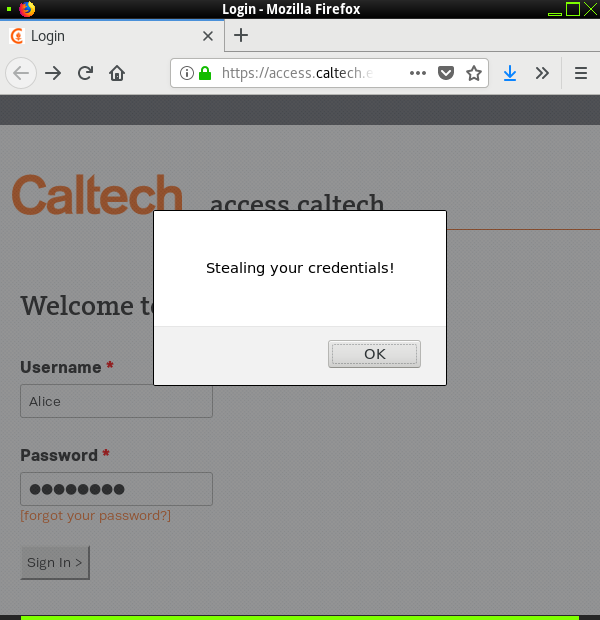
\includegraphics[width=1.2\textwidth,right]{caltech_alice}
\end{column}
\end{columns}
\end{frame}
\note{
}

%%%%%%%%%%%%%%%%%%%%%%%%%%%%%%%%%%%%%%%%%

\begin{frame}[fragile]
\frametitle{Tampering with the WAA's session tracking mechanism}
\framesubtitle{Brute force attack against the HMAC-SHA1 ``signature''}
\setlength{\parskip}{1.0em}
\begin{columns}[T]
\begin{column}[T]{0.6\textwidth}	
\setlength{\parskip}{1.0em}

\begin{enumerate}
\setlength{\parskip}{1.0em}
\item MAC generated using HMAC-SHA1
\item Secret key chosen by WAA operator
\item Weak keys present opportunity for brute force attack
\end{enumerate}
\end{column}

\begin{column}[T]{0.4\textwidth}
\begin{lstlisting}[breaklines=true, frame=single, language=Bash, xleftmargin=\parindent, basicstyle=\tiny, showstringspaces=false, linewidth=1.0\textwidth]
#!/bin/bash
data="3!200!!20180319T000000Z!20180319T000000Z!86400!0000000000-0000-0!test0001!current!pwd!!"
raw_sig="o88E6CrefqXsgfAlmePJlE0A3Tw_"
decoded_sig=$(echo $raw_sig | tr "\-._" "+/=" | base64 --decode | xxd -p)
while read key; do
    sig=$(echo -n $data | openssl dgst -sha1 -hmac $key | cut -d' ' -f2)
    echo $sig
    if [ "$sig" == "$decoded_sig" ]; then
        echo "Key found: $key"
        break
    fi
done < wordlist
\end{lstlisting}

\end{column}
\end{columns}

\end{frame}
\note{
}

%%%%%%%%%%%%%%%%%%%%%%%%%%%%%%%%%%%%%%%%%

\begin{frame}[fragile]
\frametitle{Tampering with the WAA's session tracking mechanism}
\framesubtitle{Brute force attack against the HMAC-SHA1 ``signature''}
\setlength{\parskip}{1.0em}
\begin{columns}[T]
\begin{column}[T]{1.0\textwidth}	
\setlength{\parskip}{1.0em}

\begin{enumerate}
\setlength{\parskip}{1.0em}
\item Lesson is to avoid leaving key generation to end user
\item Auto-generate key on WAA installation
\item Use slow hash algorithm to mitigate against brute force attack
\end{enumerate}
\end{column}

\begin{column}[T]{0.0\textwidth}
\end{column}
\end{columns}

\end{frame}
\note{
}

%%%%%%%%%%%%%%%%%%%%%%%%%%%%%%%%%%%%%%%%%

\begin{frame}
\frametitle{Discussion}
\framesubtitle{}
\setlength{\parskip}{1.0em}
\begin{columns}[T]
\begin{column}[T]{1.0\textwidth}	
\setlength{\parskip}{1.0em}

\begin{enumerate}
\setlength{\parskip}{1.0em}
\item Ucam Webauth is one of many SSO protocols
\item Yale's CAS is open source and more widely used
\item Stanford's WebAuth deprecated in favour of SAML 2.0
\item Open redirects present a risk for Ucam Webauth
\item Ucam Webauth remains very easy to deploy
\end{enumerate}
\end{column}

\begin{column}[T]{0.0\textwidth}
\end{column}
\end{columns}

\end{frame}
\note{
}

%%%%%%%%%%%%%%%%%%%%%%%%%%%%%%%%%%%%%%%%%

\begin{frame}
\frametitle{Conclusion}
\framesubtitle{}
\setlength{\parskip}{1.0em}
\begin{columns}[T]
\begin{column}[T]{1.0\textwidth}	
\setlength{\parskip}{1.0em}

\begin{enumerate}
\setlength{\parskip}{1.0em}
\item Raven presents a case study of security failings
\item Yet has had surprising longevity
\item Mix of protocol and implementation vulnerabilities
\item Main lessons: data sanatization, consistent security across all messages, treat error messages as security-relevant, avoid leaving key choice to end user
\item Have developed nginx implementation to address issues
\end{enumerate}
\end{column}

\begin{column}[T]{0.0\textwidth}
\end{column}
\end{columns}

\end{frame}
\note{
}

%%%%%%%%%%%%%%%%%%%%%%%%%%%%%%%%%%%%%%%%%


%%%%%%%%%%%%%%%%%%%%%%%%%%%%%%%%%%%%%%%%%
%%%%%%%%%%%%%%%%%%%%%%%%%%%%%%%%%%%%%%%%%

\end{document}
